\documentclass[11pt]{article}
\usepackage{amsmath, amssymb}
\usepackage{geometry}
\geometry{margin=1in}
\usepackage{fancyhdr}
\usepackage{lastpage}
\usepackage{parskip} % Better paragraph spacing
\usepackage{titlesec} % Better section formatting
\usepackage{graphicx}
\usepackage{float}

% Define commands for reusable content
\newcommand{\coursename}{COM-402 Information Security and Privacy}
\newcommand{\lecturenum}{01}
\newcommand{\lecturedate}{08/09/2025}
\titlespacing*{\section}{0pt}{2ex plus 1ex minus .2ex}{1.5ex plus .2ex}
% Header / Footer
\pagestyle{fancy}
\fancyhf{}
\fancyhead[L]{\coursename}
\fancyhead[R]{Lecture \lecturenum}
\fancyfoot[L]{EPFL - Computer Science}
\fancyfoot[C]{Author: Jonathan Dutoit}
\fancyfoot[R]{Page \thepage\ of \pageref{LastPage}}

\begin{document}

\begin{center}
  {\large EPFL - Computer Science} \\[0.5em]
  {\Large \textbf{\coursename}} \\[0.5em]
  {\large Lecture \lecturenum\  ---  \lecturedate} \\[0.5em]
  {\large Author: Jonathan Dutoit} \\
\end{center}

\vspace{2cm}

\begin{center}
  {\LARGE \textbf{Introduction}}
\end{center}

\vspace{1cm}

This course is a broad overview class for security and privacy.
\section*{Exercices and Homeworks}
An exercise sheet is distributed each week with both theoretical and practical questions about the lecture (including some coding exercises).

They are similar style as the exam questions. Solution sheet is distributed on Wednesday afternoon (5pm)

\section*{Quizzes}
After each major block, we release a quiz with multiple choice questions about the homework and lectures. 

Questions may be practical (i.e., homework related) or related to the lectures. 

\textbf{Recommendation:}They recommend we do it whenever they come out and try to do a serious attempts.

\section*{Course Agenda}

% Quick centered image
\begin{figure}[H]
    \centering
    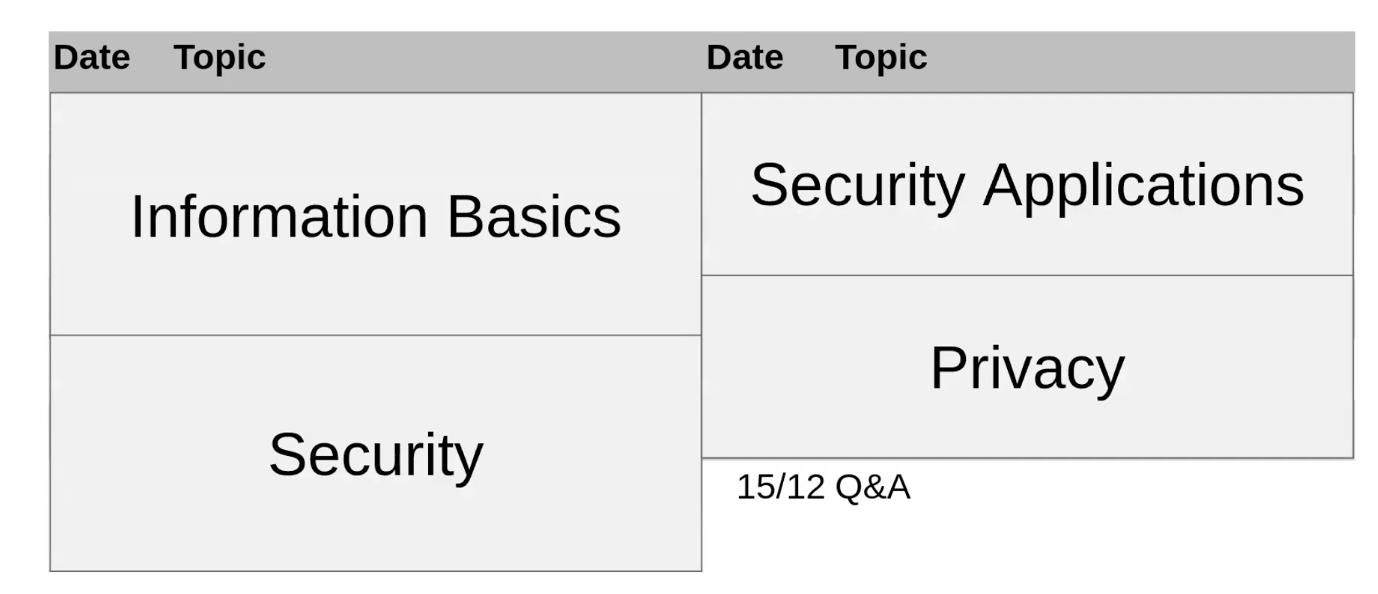
\includegraphics[width=0.7\textwidth]{course-agenda}
    \caption{Course Agenda separeted by different themes}
    \label{fig:LABEL}
\end{figure}

\section*{Information basics}
\begin{itemize}
	\item Cyber threats
	\item Crypto Basics
	\item Access Control
\end{itemize}

\section*{Security}
\begin{itemize}
	\item Data Security
	\item Programming Language Security and Compartments
	\item OWASP and Software Security
\end{itemize}

\section*{Security Applications}
\begin{itemize}
	\item Automated Testing / Fuzzing
	\item Mobile Security (Android as example)
	\item Network and Operations Security
	\item TEEs and Side Channels
\end{itemize}

\section*{Privacy}
\begin{itemize}
	\item Privacy
	\item Machine Learning Security and Privacy
\end{itemize}

\section*{Summary}

Security and privacy is about controlling risk

You can't be secure without: 
\begin{itemize}
	\item knowing your assets, threats, and risks
	\item have some basic trust assumptions (e.g., encryption cannot be broken, my sysadmin is honest, etc.) 
\end{itemize}

Solved by defining a policy, selecting mechanisms and implementing them (in practice much harder than it sounds) 

Security is an \textbf{ongoing process}, requires regular audit/improvement

\end{document}
